\chapter{Architecture}
\label{chap:architecture}

\section{Overview}
The platform follows a layered architecture. The ingestion layer collects explicitly authorised sources. The processing layer validates, normalizes and chunks documents. The intelligence layer extracts entities and relations with Mistral and creates NVIDIA embeddings. The storage layer combines a raw zone, a graph store and a vector index. Finally, FastAPI exposes the services to a React interface.

\begin{figure}[H]
\centering
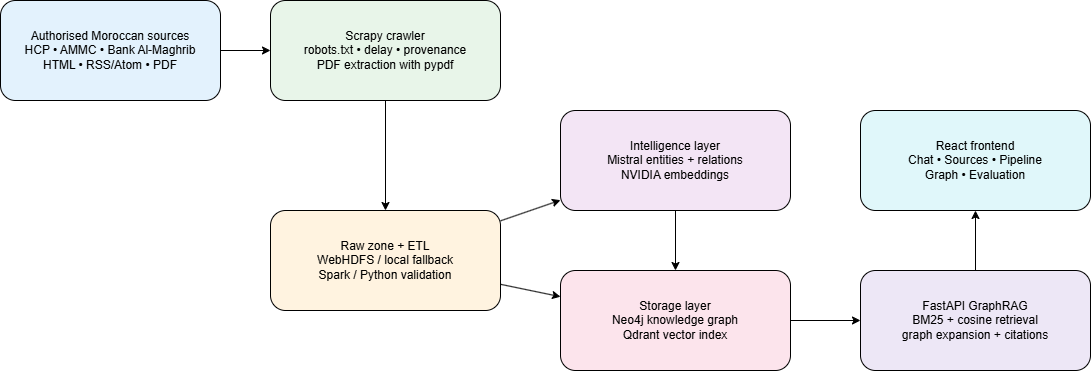
\includegraphics[width=\textwidth]{images/00-general-architecture.png}
\caption{General architecture of the Moroccan GraphRAG platform.}
\label{fig:general-architecture}
\end{figure}

\section{Information Flow}
The flow is: source URL $\rightarrow$ Scrapy item $\rightarrow$ raw document $\rightarrow$ Spark/Python ETL $\rightarrow$ chunks $\rightarrow$ graph and vector indexes $\rightarrow$ GraphRAG retrieval $\rightarrow$ cited answer. Each page keeps its URL, domain, title, language, document type and crawl timestamp.

\section{Deployment}
Docker Compose runs the API, frontend, ingestion worker, Qdrant and Neo4j. WebHDFS and Spark are optional integrations with local fallbacks for development. This keeps the prototype executable on a workstation while preserving a path to distributed deployment.

\begin{figure}[H]
\centering
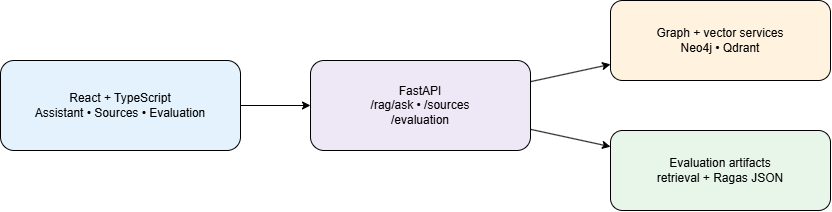
\includegraphics[width=0.9\textwidth]{images/06-frontend-compose.png}
\caption{Frontend, API and service deployment view.}
\label{fig:deployment}
\end{figure}

\section{Current Corpus and Target Sources}
The current indexed corpus contains \textbf{48 documents}: 35 HTML pages, 10 RSS/Atom entries and 3 PDF documents. The documents come from three domains: HCP (24), AMMC (16) and Bank Al-Maghrib (8). The configured targets are the HCP enterprise and economy pages, the AMMC issuer financial-statements page, Bank Al-Maghrib statistics, the Bank Al-Maghrib annual report PDF and the HCP RSS feed.
